\documentclass{article}
\usepackage[utf8]{inputenc}

\title{Hw3 Report}
\author{Muhammed Yasir Fidan }
\date{April 2021}

\usepackage{natbib}
\usepackage{graphicx}

\begin{document}

\maketitle

\section{Abstract}
Firstly, My program only works fine for 2 processes, one process has potato and other one not in the beginning. If there are more than 2 processes program stuck in a deadlock. When program starts
They exchange potato between their fifos and there is a shared memory for track potato switch and ensure both process dont try to create same fifo. The semaphore I take as argument used protect shared memory to block access two process at the same time. Also I create a second semophore. This semaphore used for making the potato process is waiting for the non-potato process to create its fifos first. If there is not this semaphore, sometimes potato process can reach sending potato case before non-potato process create his fifo, so potato process cant find fifo. For solving this I use this semaphore.


\section{Compile And Running}
For compiling just use makefile, enter make. In makefile I use -Wall flag too so there is no warning when compiling as you can see.

\begin{figure}[h!]
\centering
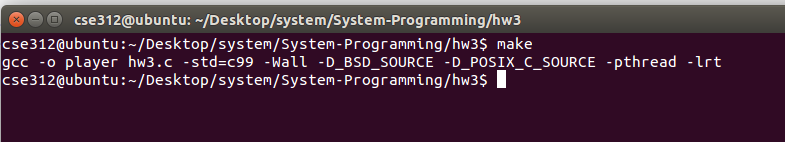
\includegraphics[scale=0.5]{hw_3.png}
\caption{compile}
\label{fig:compile}
\end{figure}

For running execute 2 program by using & in terminal. For example here I execute 2 program they have exacly same parameter but one of them -b 10 and other 0. This means -b 10 has a potato that must switch 10 times and other process start without a potato.
\newpage

\begin{figure}[h!]
\centering
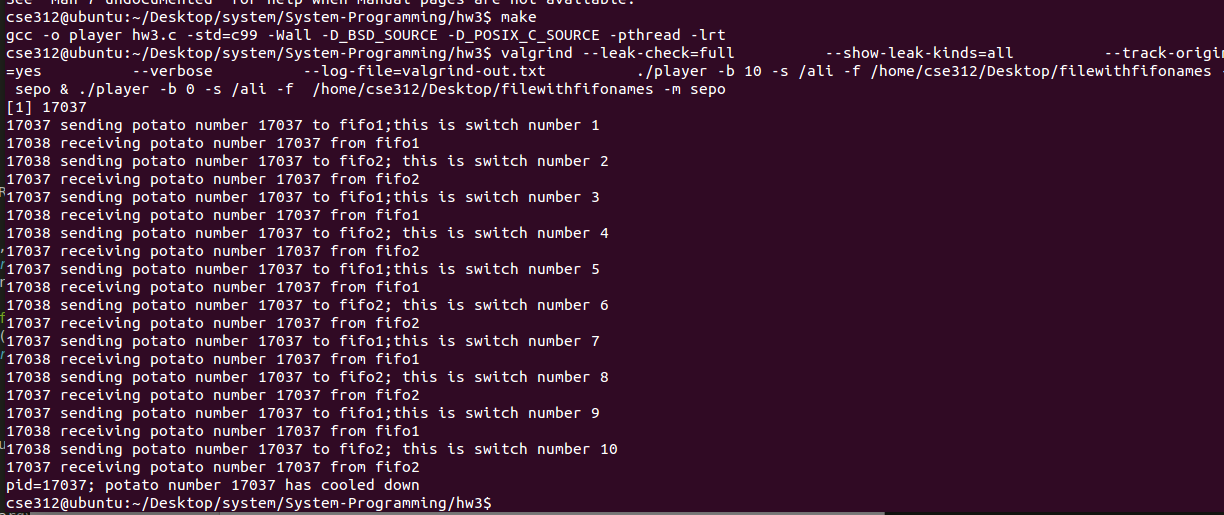
\includegraphics[scale=0.35]{hw3_1.png}
\caption{running}
\label{fig:running}
\end{figure}

Here as you can see processes send potato each other 10 times because -b argument is 10. Then it print potato cool down and both process end. For this running my shared memory name /ali, my semaphore name sepo and -f shows fifo file path.
This is my fifo file, here there is 2 fifo path. So my program create this fifos under those paths when my program executed.

\begin{figure}[h!]
\centering
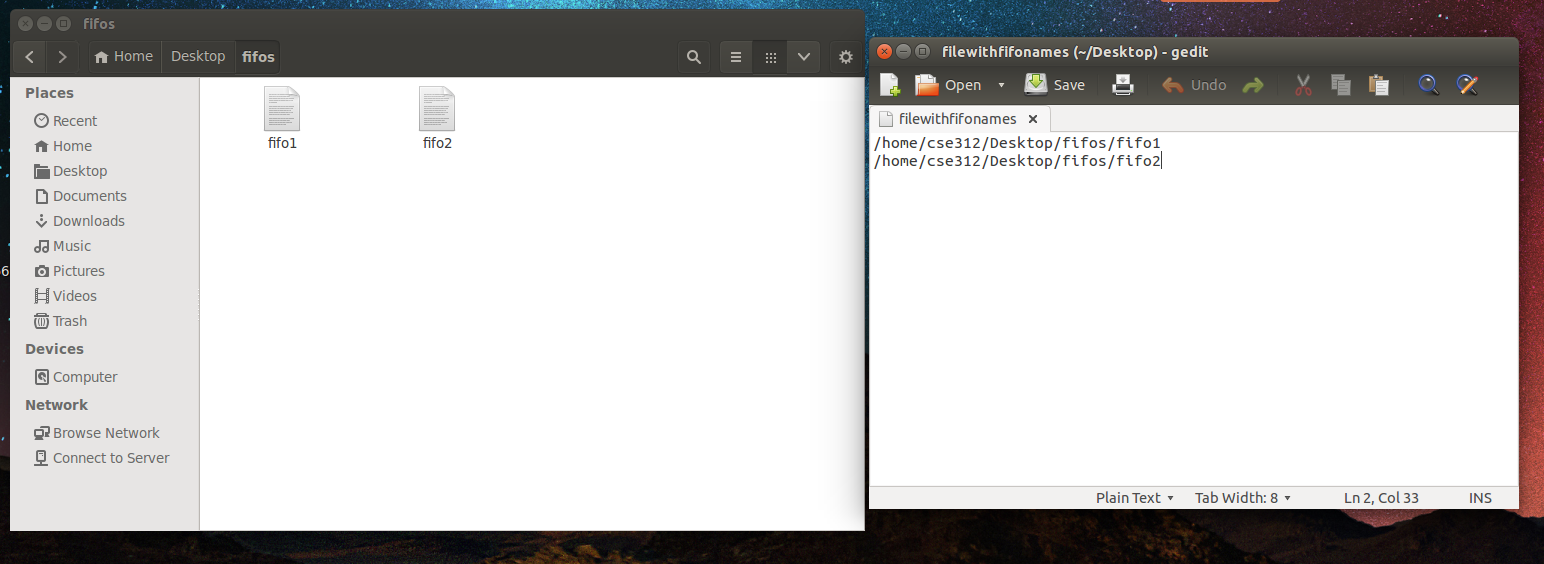
\includegraphics[scale=0.3]{hw3_4.png}
\caption{fifo file}
\label{fig:running}
\end{figure}

\newpage

\begin{figure}[h!]
\centering
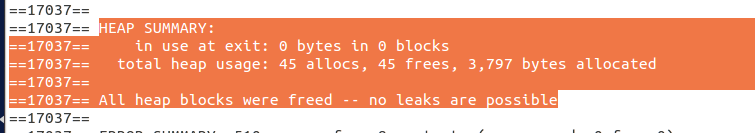
\includegraphics[scale=0.35]{hw3_2.png}
\caption{Valgrind memory leak}
\label{fig:running}
\end{figure}

And in valgrind output there is no memory leak.

\end{document}
